\chapter{Discussion}

In the first chapter, we established that reading utilizes a variety of cognitive skills whose neural substrates are distributed throughout the brain. But being able to comprehend speech is a pre-requisite to reading, and it is similarly complex. This begs the question: in what ways is reading unique from listening?

A connectomics approach to reading illuminates -- not displaces -- previous neuroimaging research, much of which focused on localizing specific cognitive processes.

The most widely-held view is that reading and listening share the same core linguistic processes and differ primarily in the sensory processes that feed into supra-model linguistic systems \citep{Mattingly1971, Price2012}. One popular model, the \textit{Simple View of Reading} states that reading comprehension is the product of listening comprehension and decoding skills \citep{Gough1986}. This view has received support from large behavioral studies \citep{Kirby2008} and neuroimaging investigations: many of the literacy-related changesare linked to visual or phonological systems, areas not directly related to semantic or comprehension processes \citep{Schlaggar2007, Dehaene2015}. These findings support a model in which inputs from auditory or visual domains are fed up into higher-order association areas that sequence, encode articulatory plans, and extract semantic information \citep{Price2012}. These processes localize onto the similar areas regardless of language and writing system \citep{Rueckl2016}, and may even extend to inputs from somatosensory domains \citep{Xu2005, Sood2016}. This supra-modal language core is largely left-lateralized and centers on the inferior frontal gyrus, anterior and posterior middle temporal gyrus and the angular gyrus. Neuroanatomical models of language, shown in Fig. \ref{ch3-price-language-models}, illustrate that language is distributed throughout much of the brain. 

\begin{figure}[t]
	\centering
	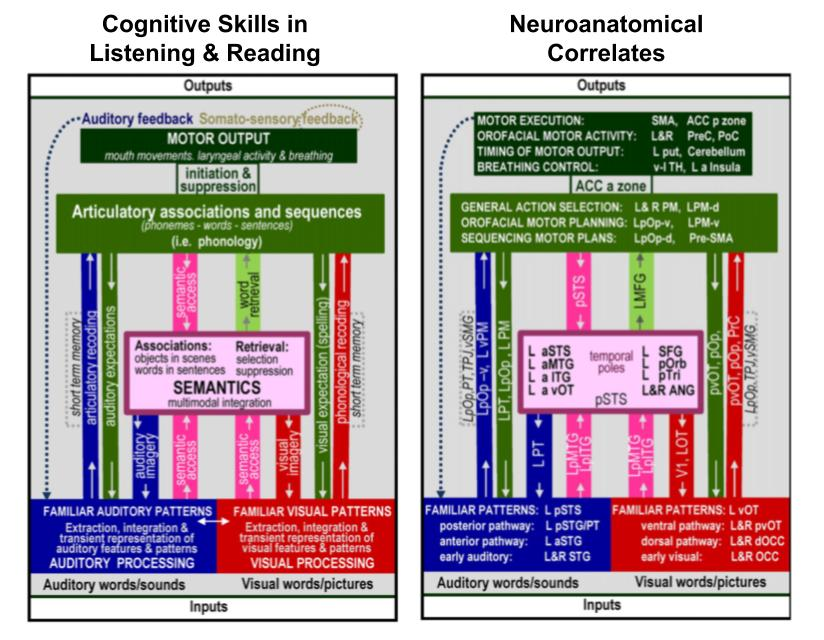
\includegraphics[height=3in]{images/ch3-price-language-models.jpg}
	\caption[Schematics of skills and brain areas used in reading.]{Models of reading typically focus on a common linguistic core that is responsible for comprehension and production of language. In this model, differences in modality affect input pathways to this core.}
	\label{fig:ch3-price-language-models}
\end{figure}


In this study, we pursue three hypothesized ways reading might differ from listening. These are not exclusive; one or more of them may be true. The overarching aim is to test whether reading and listening differ only, or primarily, in their 

\begin{itemize}
	\item Reading will require a greater global reorganization of resting-state networks than listening. This network will also be more highly integrated than that of listening. 
	\item Reading will reduce the modularity within the sensory system of interest. That is, visual areas will become less internally connected during reading, while auditory areas will be less internally connected during listening.
	\item Reading will make greater demands on attention systems than listening. That is, areas in the frontal and attention systems will be activated to a greater degree during reading than listening.
\end{itemize}

%%%%


\citep{Petersen2016}


\section{Dynamic modeling of network architecture}

We could use dynamic modeling....

\section{Individualized parcellations}

A caveat with connectomics analyses, including those presented here, are that results for the modularity analyses are often based on RSN parcellations from previous literature \citep{Power2011}. It is possible that in this sample of children, there were differences in network organization that resulted in a lower global modularity but were in fact due to differences in organization (e.g. multiple sub-modules of the default mode network). The question of how network architecture develops over time, and how best to measure it is under active investigation \citep{Cao2016}. Its answer will have important implications for disentangling this complex interchange between development, network architecture and cognitive performance.



\section{Multi-modal investigations}


% Fronto-parietal description
% Task-based neuroimaging provides us with a rich description of the functions of frontoparietal network. The frontoparietal network is an assembly of brain regions encompassing the lateral frontal and parietal cortices along with insular, anterior/mid cingulate, and inferior temporal areas that have been broadly implicated in a variety of higher-level cognitive tasks \citep{Fedorenko2013}. Some have described the frontoparietal network as supporting active and adaptive online control, initiating and adjusting goal-directed mental systems \citep{Dosenbach2007}, while others have proposed a more general superordinate role in directing cognition \citep{Niendam2012}. The most obvious relationship of the frontoparietal network to language is its proximity to Broca’s area, known for its critical role in language articulation. Rather than thinking of this area (traditionally, Brodmann areas 44 and 45) as exclusively or primarily language-related, it has been argued that Broca’s area supports hierarchical executive processing, such as the segmentation (``chunking'') of auditory language and the flexible combination of words \citep{Koechlin2006}. Thus, while Broca's area plays a role in the unification of representations, prefrontal cortex (and the larger frontoparietal network) may play a higher-level control and initiating role in language and other processes \citep{Hagoort2005}. 

% Right hemisphere
% Our findings show that in stronger readers, the left frontoparietal RSN is expanded to include portions of the right posterior middle and superior temporal cortex.  These regions may play a number of roles in more skilled readers.  First, these right hemisphere regions are homologues of important left hemisphere language areas. The left posterior superior and middle temporal gyri are major secondary processing areas for written and auditory word stimuli \citep{Price2012}. In the right hemisphere, these areas are understood to play a complementary role, with a sensitivity to both emotional and prosodic elements \citep{Jung-Beeman2005}. Thus, the expansion of the frontoparietal network to these homologues could represent greater ``recruitment'' of complimentary language areas, facilitating  the integration of language-related information.  Secondly, these right hemisphere areas are subregions of the generally bilateral ventral attention RSN \citep{Yeo2011}.  Nonetheless in task-based studies, this network shows more of a right-sided bias \citep{Fox2006}.  As such, good readers may be better at integrating visual information with more high-order information.  These explanations need not be mutually exclusive.

% Ventral attention network
% While we found an expansion of the left frontoparietal RSN to regions of the ventral attention RSN in good readers, we did not find an association between variation in the ventral attention RSN itself and individual differences in reading ability. The ventral attention network detects salient or unexpected stimuli in the environment \citep{Vossel2014}. In this way the ventral attention network can act as a ‘circuit breaker’ for the dorsal system to help reorient attention \citep{Corbetta2002}. It may thus help orient individuals to new information from the visual environment (i.e. text) and, by coupling stimulus-driven attentional areas with the frontoparietal network, it may help construct updated mental representations of linguistic material. The leftward aspects of the ventral attention network underlie crucial reading-related areas, including occipito-temporal cortex, which performs orthographic processing, and temporo-parietal cortex, important for semantic binding \citep{Taylor2013}. The absence of reading-related variance associated with the entire bilateral RSN may reflect the diversity of functions that these areas serve in basic visual and auditory processing, as well as language and reading. 

